\documentclass[12pt,a4paper]{report}
\usepackage[english]{babel}
%\usepackage{newlfont}

%%\usepackage{amsfonts}
\usepackage{amssymb}
\usepackage{hyperref}
\usepackage{bm}
\usepackage{graphicx}
\usepackage{color}
\usepackage{tikz}
\usetikzlibrary{arrows}

\usepackage{pdfpages}

\usepackage{bm}
\usepackage{newlfont}
\usepackage{color}
\textwidth=450pt\oddsidemargin=0pt
\usepackage{systeme}

\newcommand{\facciatabianca}{\newpage\shipout\null\stepcounter{page}}

\newcommand{\xtodo}[2][]{\tikzexternaldisable\todo[#1]{#2}\tikzexternalenable}
\usepackage{fancyhdr}

\usepackage{indentfirst}
\usepackage{graphicx}
\usepackage{newlfont}

\usepackage{amssymb}
\usepackage{amsmath}
\usepackage{latexsym}
\usepackage{amsthm}
%
%\oddsidemargin=30pt \evensidemargin=20pt%impostano i margini
\hyphenation{}                          %serve per la sillabazione
\theoremstyle{plain}                    %stile corsivo
\newtheorem{teo}{Teorema}[section]      %definizione ambiente teorema
\newtheorem{prop}[teo]{Proposizione}    %definizione ambiente proposizione
\newtheorem{cor}[teo]{Corollario}       %definizione ambiente corollario
\newtheorem{lem}[teo]{Lemma}            %definizione ambiente lemma
\theoremstyle{definition}               %stile roman
\newtheorem{defin}{Definizione}[chapter]%definizione ambiente definizione
\newtheorem{ese}{Esempio}[chapter]      %definizione ambiente esempio
\theoremstyle{remark}                   %stile per osservazioni
\newtheorem{oss}{Osservazione}          %definizione ambiente osservazione
%%%%%%%%%%%%%%%%%%%%%%%%%%%%%%%%%%%%%%%%%comandi per l'impostazione
                                        %   della pagina, vedi il manuale
                                        %   della libreria fancyhdr
                                        %   per ulteriori delucidazioni
\pagestyle{fancy}\addtolength{\headwidth}{20pt}
\renewcommand{\chaptermark}[1]{\markboth{\thechapter.\ #1}{}}
\renewcommand{\sectionmark}[1]{\markright{\thesection \ #1}{}}
\rhead[\fancyplain{}{\bfseries\leftmark}]{\fancyplain{}{\bfseries\thepage}}
\cfoot{}
%%%%%%%%%%%%%%%%%%%%%%%%%%%%%%%%%%%%%%%%%
\linespread{1.3}                        %comando per impostare l'interlinea
%%%%%%%%%%%%%%%%%%%%%%%%%%%%%%%%%%%%%%%%%definisce nuovi comandi
\newcommand{\df}{\displaystyle\frac}    %crea un comando che visualizza le
                                        %   frazioni in modo più esteso
\newcommand{\seq}[1]{\left<#1\right>}   %crea un comando per il "generato"
                                        %   di un insieme, per richiamarlo
                                        %   si può scrivere ad esempio:
                                        %           $\seq{q_1,q_2}$
\begin{document}


\begin{titlepage}

\begin{center}
{{\Large{\textsc{Alma Mater Studiorum $\cdot$ Universit\`a di Bologna}}}} 
\rule[0.1cm]{15.8cm}{0.1mm}
\rule[0.5cm]{15.8cm}{0.6mm}
\\\vspace{3mm}

{\small{\bf Scuola di Scienze \\ 
Dipartimento di Fisica e Astronomia\\
Master in Physics}}

\end{center}

\vspace{23mm}
\begin{center}
\vspace{3mm}
{\LARGE{\bf }}
\vspace{3mm}
{\LARGE{\bf }}
\\
\end{center}
\vspace{40mm}
\par
\noindent
\begin{minipage}[t]{0.47\textwidth}
{\large{\bf Relatore:\\
Prof.\\
Armando Bazzani}}
\end{minipage}
\hfill
\begin{minipage}[t]{0.47\textwidth}\raggedleft
{\large{\bf Presentata da:\\
Riccardo Scheda}}
\end{minipage}
\vspace{30mm}
\begin{center}
{\large{\bf Anno Accademico 2017-2018}}
\end{center}
\end{titlepage}



\facciatabianca

\chapter*{Abstract}

Real living cell is a complex system governed by many process which are not yet understood: the process of cell differentiation is one of these. 
Cell  differentiation is the process in which cells of a specific type reproduces themselves and give arise to different type of cells.
Cell differentiation is governed by the so called Gene Regulatory Networks (GRNs).
A GRN is a collection of molecular regulators that interact with each other and with other substances in the cell to govern the gene expression levels of mRNA and proteins. 
Kauffman proposed for the first time in 1969 to model GRN through the so called Random Boolean Networks (RBN).
RBNs are networks in which each node can have only two possible values: 0 or 1, where each node represent a gene in GRN which can be "on" or "off".
These networks can model GRNs because the activity of one node represents the expression level of one gene among the whole regulation.

In this thesis work we make use of a mathematical model to develop and reproduce a possible Gene Regulatory Network for the process of cell differentiation.


%%%%%%%%%%%%%%%%%%%%%%%%%%%%%%%%%%%%%%%%%non numera l'ultima pagina sinistra
\clearpage{\pagestyle{empty}\cleardoublepage}

\tableofcontents                        %crea l'indice
%%%%%%%%%%%%%%%%%%%%%%%%%%%%%%%%%%%%%%%%%imposta l'intestazione di pagina
\rhead[\fancyplain{}{\bfseries\leftmark}]{\fancyplain{}{\bfseries\thepage}}
\lhead[\fancyplain{}{\bfseries\thepage}]{\fancyplain{}{\bfseries
INDICE}}

%%%%%%%%%%%%%%%%%%%%%%%%%%%%%%%%%%%%%%%%%non numera l'ultima pagina sinistra
\clearpage{\pagestyle{empty}\cleardoublepage}
\listoffigures                          %crea l'elenco delle figure
%%%%%%%%%%%%%%%%%%%%%%%%%%%%%%%%%%%%%%%%%non numera l'ultima pagina sinistra



\chapter*{Introduction}                 %crea l'introduzione (un capitolo
                                        %   non numerato)
%%%%%%%%%%%%%%%%%%%%%%%%%%%%%%%%%%%%%%%%%imposta l'intestazione di pagina
\rhead[\fancyplain{}{\bfseries
INTRODUCTION}]{\fancyplain{}{\bfseries\thepage}}
\lhead[\fancyplain{}{\bfseries\thepage}]{\fancyplain{}{\bfseries
INTRODUCTION}}
%%%%%%%%%%%%%%%%%%%%%%%%%%%%%%%%%%%%%%%%%aggiunge la voce Introduzione
                                        %   nell'indice
\addcontentsline{toc}{chapter}{Introduction}



\chapter{Cell Differentiation }\label{celldiff}
\lhead[\fancyplain{}{\bfseries\thepage}]{\fancyplain{}{\bfseries\rightmark}}

In this Chapter we explain Cell Differention process and Gene Regulatory Networks.

\section{Definition}
Cell differentiation is the process whereby stem cells become progressively
more specialized. The differentiation process occurs both during the development of a multicellular organism and during tissue repair and cell turnover
in the adulthood. Gene expression, and therefore its regulatory mechanisms,
plays a critical role in cell differentiation.
\begin{figure}
\centering
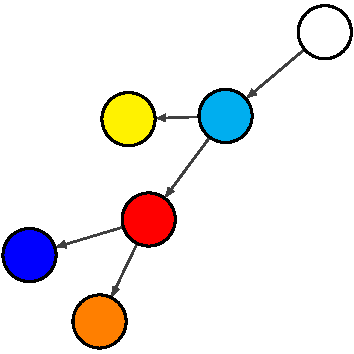
\includegraphics[angle=45]{images/cells.pdf}
\caption{\emph{Schematic representation of cellular differentiation.}}
\end{figure}
Stem cells are undifferentiated biological cells which can both reproduce
themselves, self-renewal ability, and differentiate into specialized cells, potency.
The principles underlying cellular differentiation remain among the most
enigmatic in biology. We are required to explain the spontaneous generation of a multiplicity of cell types from the single zygote, to deduce a natural
tendency of a system to become increasingly heterogeneous, then to stop
differentiating.

Among the important characteristics of cell differentiation are: 
\begin{itemize}
\item initiation
of change; 
\item stabilization of change after cessation of stimulus; 
\item the efficacy of
many substances, exogenous and endogenous, as inductive stimuli;
\item progressive limitation in the number of developmental pathways open to any small region of the embryo; 
\item restricted periods during which
a cell is competent to respond to an inductive stimulus; the discreteness of
cell types, that is, the mutually exclusive constellations of properties by
which cells differ; 
\item a requirement for a minimal and preferably heterogeneous
cell mass to initiate differentiation in many instances, and to maintain it in
some; 
\item the occurrence of metaplasia between undifferentiated cell types, or
from an undifferentiated type to a specialized type, but the lack of metaplasia
(the isolation) between specialized cell types; 
\item cessation of differentiation.
\end{itemize}

Cells are thought to differ due to differential expression of, rather than
structural loss of, the genes. Differential activity of the genes raises at least
two questions which are not always carefully distinguished: the capacity of
the genome to behave in more than one mode; and mechanisms which insure
the appropriate assignment of these modes to the proper cells.



Within multicellular organisms, tissues are organized in communities of cells that work together to carry out a specific function. The exact role of a tissue in an organism depends on what types of cells it contains. For example, the endothelial tissue that lines the human gastrointestinal tract consists of several cell types. Some of these cells absorb nutrients from the digestive contents, whereas others secrete a lubricating mucus that helps the contents travel smoothly.
However, the multiple cell types within a tissue don't just have different functions. They also have different transcriptional programs and may well divide at different rates. Proper regulation of these rates is essential to tissue maintenance and repair. 
Stem cells typically have the capacity to mature into many different cell types. \emph{Transcription factors} (TF), which are proteins that regulate which genes are transcribed in a cell, appear to be essential to determining the pathway particular stem cells take as they differentiate. For example, both intestinal absorptive cells and goblet cells arise from the same stem cell population, but divergent transcriptional programs cause them to mature into dramatically different cells.
Whenever stem cells are called upon to generate a particular type of cell, they undergo an asymmetric cell division. With asymmetric division, each of the two resulting daughter cells has its own unique life course. In this case, one of the daughter cells has a finite capacity for cell division and begins to differentiate, whereas the other daughter cell remains a stem cell with unlimited proliferative ability.

\section{The role of Gene expression in cellular differentiation}
Gene expression is a complex process regulated at several stages in the synthesis of proteins. In addition to the DNA transcription regulation, the expression of a gene may be controlled during RNA processing and transport (in eukaryotes), RNA translation, and the post-translational modification of proteins. This gives rise to genetic regulatory systems structured by networks of regulatory interactions between DNA, RNA, proteins and other molecules: a complex network termed as a \emph{gene regulatory
network} (GRN) (see Chapter \ref{grn}). Some kind of proteins are the transcription factors that bind to specific DNA sequences in order to regulate the
expression of a given gene. The power of transcription factors resides in their ability to activate and/or repress transcription of genes. The activation of
a gene is also referred to positive regulation, while the negative regulation
identifies the inhibition of the gene.
The regulation of gene expression is essential for the cell, because it
allows to control the internal and external functions of the cell. Furthermore,
in multicellular organisms, gene regulation drives the processes of cellular
differentiation and morphogenesis, leading to the creation of different cell
types that possess different gene expression profiles, and these last therefore
produce different proteins that have different ultrastructures that suit them
to their functions. Therefore, with few exceptions, all cells in an
organism contain the same genetic material, and hence the same genome. The difference between the cells are emergent and due to regulatory mechanisms which can turn on or off genes. Two cells are different, if they have different subsets of active genes.

%\section{Cell differentiation in Immune system}
%Cell differentiation concerns all type of cells, and in particular one of the most %important systems in the organisms: the Immune system. 
%Immune  system is a host defense system comprising many biological structures and processes %within a organims that protects against disease.
%To function properly, an immune system must detect a wide variety of agents, known as %pathogens, from viruses to parasitic worms, and distinguish them from the organism's own %healthy tissue. In many species, there are two major subsystems of the immune system: the %innate immune system and the adaptive immune system.

%Cellular differentiation concerns with immune system beacuse it is composed by a wide range %of different cells: \emph{B lymphocytes, T lymphocytes, Basophil, Eosinophil,} etc. In the %next Chapter we will concentrate on the so called \emph{T cells}, which are important for %the immune system and in particular because they are the focus of our mathematical model.


\chapter{Gene Regulatory Networks}\label{grn}
\lhead[\fancyplain{}{\bfseries\thepage}]{\fancyplain{}{\bfseries\rightmark}}


\section{Definition}

Gene regulation controls the expression of genes and, consequently, all cellular functions. Gene expression is a process that involves transcription of the gene into mRNA, followed by translation to a protein, which may be subject to post-translational modification \cite{K40}. The transcription process is controlled by transcription factors (TFs) that can work as activators or inhibitors. TFs are themselves encoded by genes and subject to regulation, which altogether forms complex regulatory networks. 
\begin{figure}
\centering
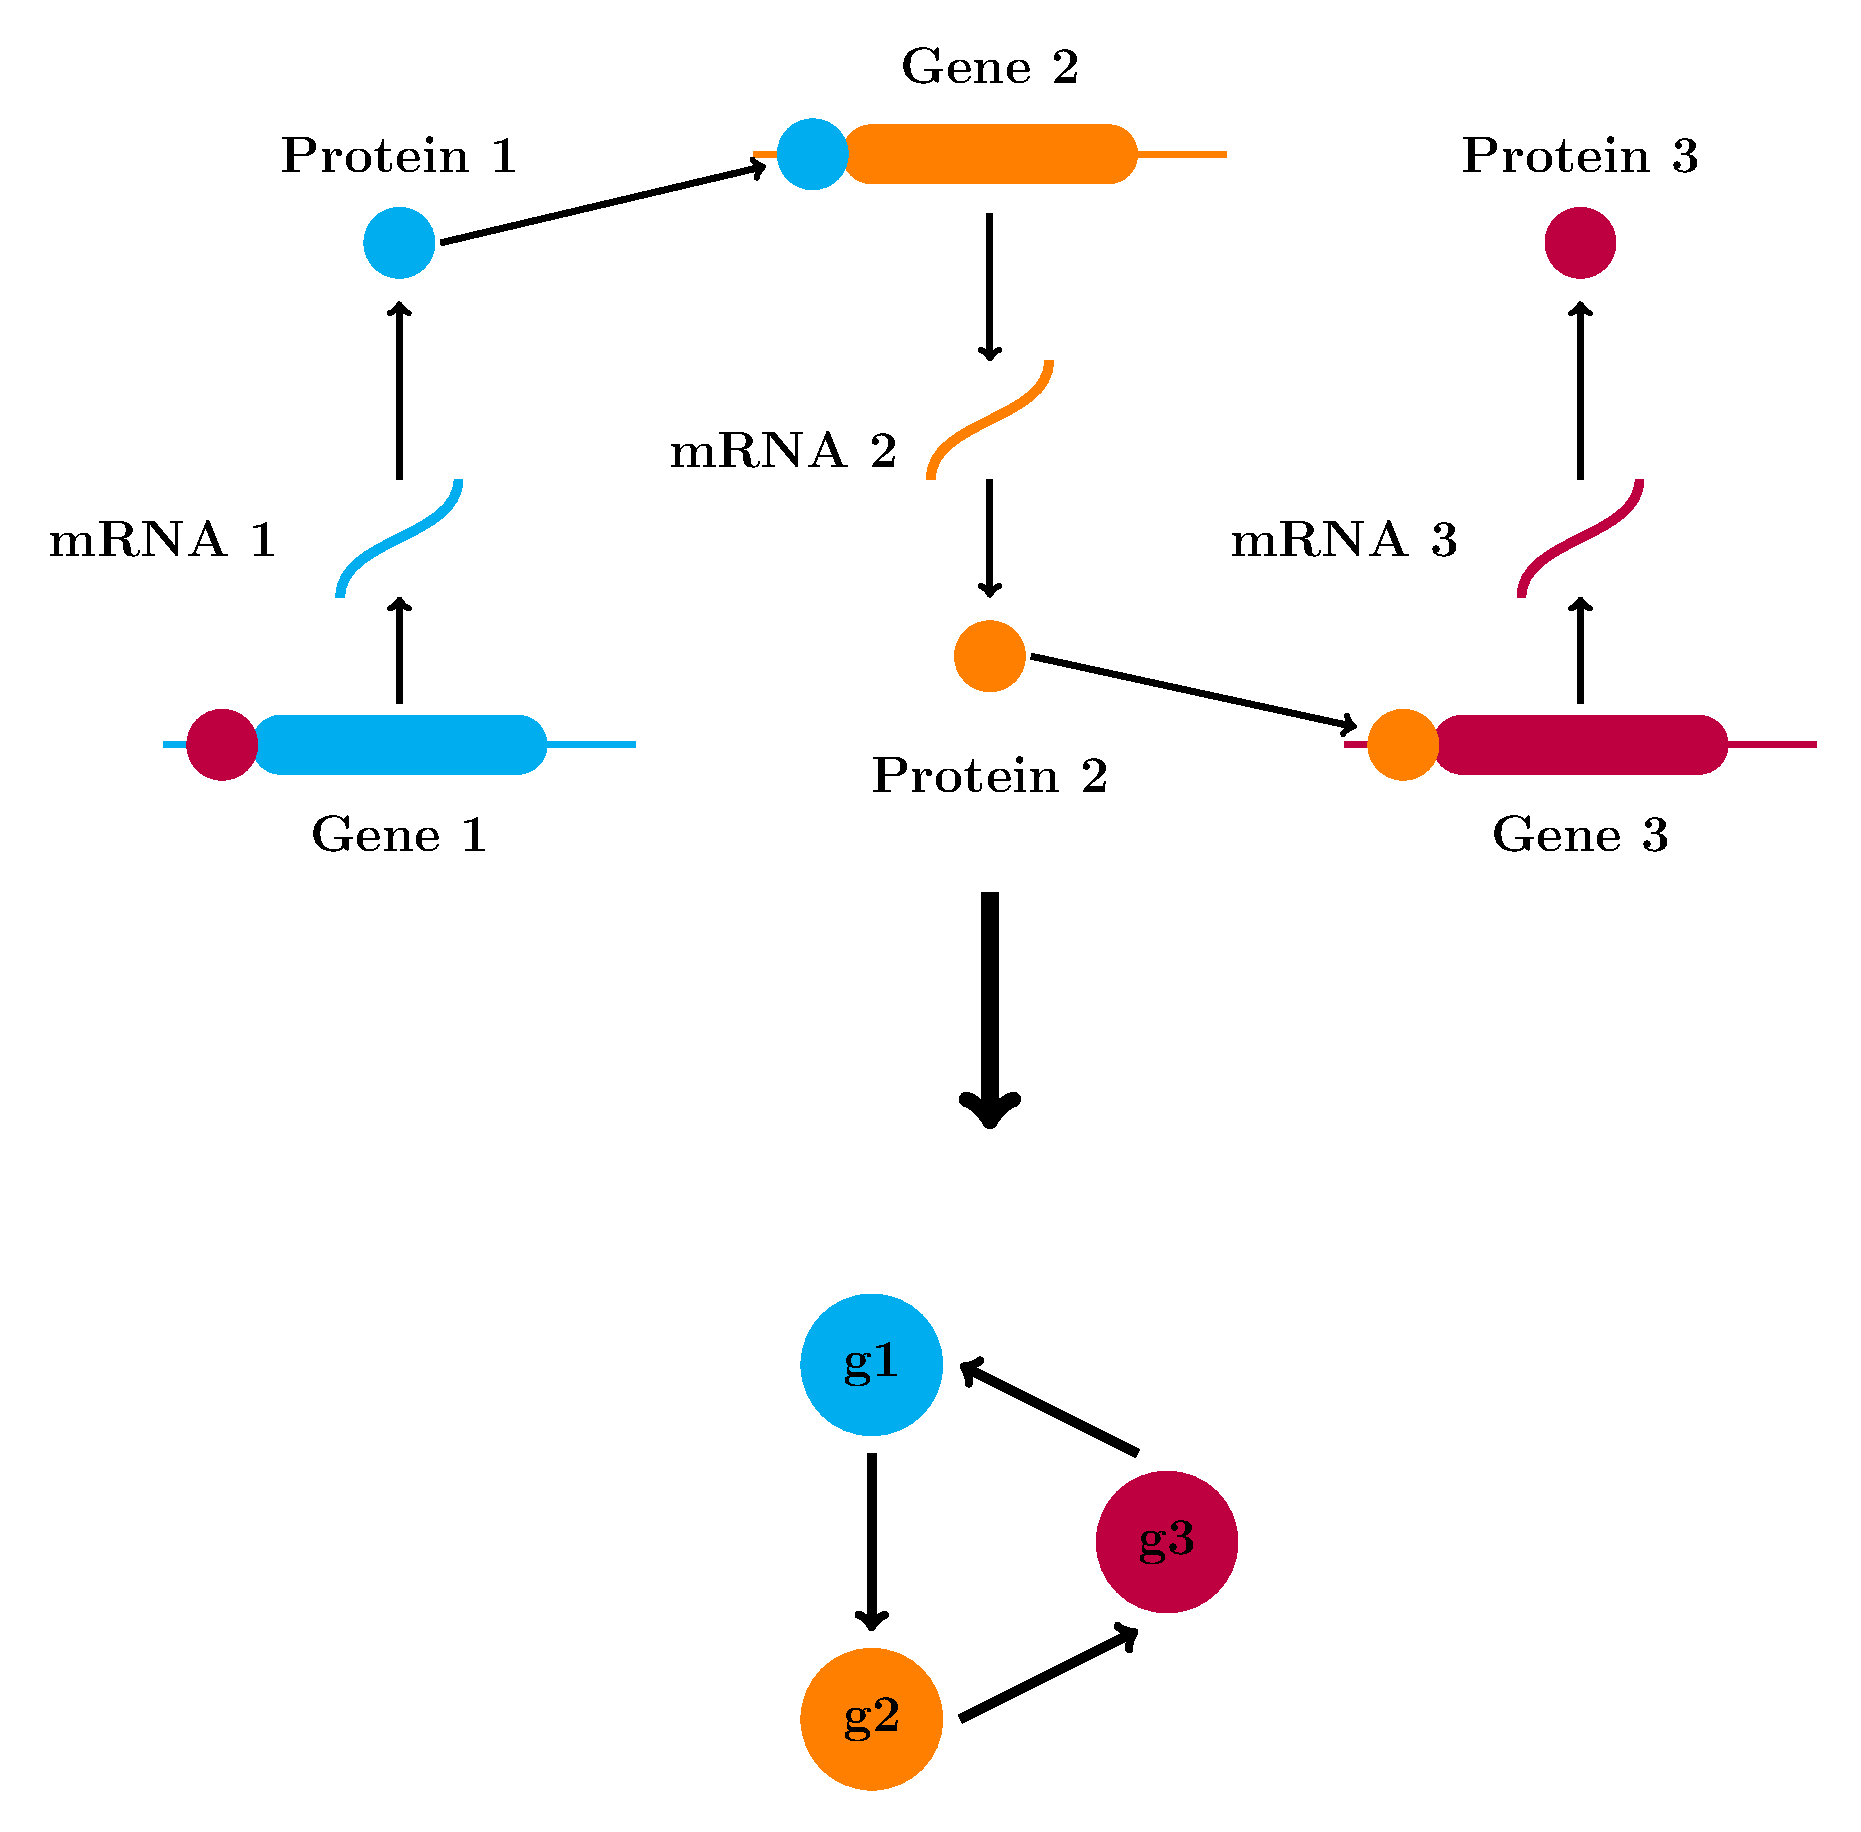
\includegraphics[scale=0.4]{images/grnn.pdf}
\caption{\emph{Schematic representation of a Gene Regulatory Network.}}
\end{figure}
Cells efficiently carry out molecular synthesis, energy transduction, and signal processing across a range of environmental conditions by networks of genes, which we define broadly as networks of interacting genes, proteins, and metabolites \cite{K37}. Formally speaking, a \emph{gene regulatory network} or \emph{genetic regulatory network} (GRN) is a collection of DNA segments in a cell which interact with each other (indirectly through their RNA and protein expression products) and with other substances in the cell, thereby governing the rates at which genes in the network are transcribed into mRNA. In general, each mRNA molecule goes on to make a specific protein (or set of proteins). In some cases this protein will be structural, and will accumulate at the cell-wall or within the cell to give it particular structural properties. 

These networks control biological process of all organisms. The complex control systems underlying development have probably been evolving for more than a billion years. They regulate the expression of thousand of genes in any given biological process. They are essentially hardwired genomic regulatory codes, the role of which is to specify the sets of genes that must be expressed in specific spatial and temporal patterns. In physical terms, these control system consist of many thousands of modular DNA sequences. Each module receives and integrates multiple inputs, in the form of regulatory proteins (\emph{activators} and \emph{repressors}) that recognize specific sequences within them. The end result is the precise transcriptional control of the associated genes. 
Functional linkages between these particular genes, and their associated regulatory modules, define the core networks underlying development. They explain exactly how genomic sequence encodes the regulation of expression of the sets of genes that generate patterns and execute the construction of multiple states of differentiation.

The regulatory genome is a logic processing system: every regulatory module contained in the genome receives multiple inputs and processes in ways that can be mathematically represented as combinations of logic functions. 

Definitive regulatory functions emerge only from the architecture of intergenic linkages, and these functions are not visible at the level of any individual genes. So gene regulatory networks can be determined only by experimental molecular biology in which the functional meaning of given regulatory sequences is directly determined.

GRNs have a complex structure: they are inhomogeneous compositions of different kinds of subnetworks, each performing a specific kind of function. Some subnetworks are used in many processes.

In principle, mathematical modeling of GRN dynamics can provide a theoretical foundation for understanding cell heterogeneity and gene expression dynamics, by quantitatively linking molecular-level regulatory mechanisms with observed cell states. However, due to the molecular complexity of gene regulatory mechanisms, it remains challenging to integrate such models with single-cell data.

\section{Modelling GRNs}
Mathematical models can account for (and at least partially reproduce) observed cellular heterogeneity in two primary ways. First, gene network models are multistable dynamical systems, meaning a given network has the potential to reach multiple stable states of gene expression. These states arise from the dynamic interplay of activation, inhibition, feedback, and nonlinearity \cite{K1} \cite{K42}. Second, some mathematical models inherently treat cellular noise. This noise, or stochasticity, is modeled in various ways depending on assumptions about the source \cite{K43} \cite{K44}. Discrete, stochastic models of gene regulation, which track discrete molecular entities, regulatory-protein binding kinetics, and binding states of promoters controlling gene activity, have formed the basis of biophysical theories of gene expression noise due to so-called intrinsic molecular noise \cite{K44} \cite{K45}. Such stochastic gene regulation mechanisms have also been incorporated into larger regulatory network models using the formalism of stochastic biochemical reaction networks, and have been utilized to explore how molecular fluctuations can cause heterogeneity within phenotype-states and promote stochastic transitions between phenotypes \cite{K46} \cite{K47}.

The quantitative landscape of cellular states is another concept that is increasingly utilized to describe cellular heterogeneity. Broadly, the cellular potential landscape (first conceptualized by Waddington \cite{K12}\cite{K13}) is a function in high-dimensional space (over many molecular observables, typically expression levels of different genes), that quantifies the stability of a given cell state. In analogy to potential energy (gravitational, chemical, electric, etc.), cell states of higher potential are less stable than those of lower potential. The landscape concept inherently accounts for cellular heterogeneity, since it holds that a continuum of states is theoretically accessible to the cell, with low-potential states (in “valleys”) more likely to be observed than high-potential states. The landscape is a rigorously defined function derived from the dynamics of the underlying gene network model, according to some choice of mathematical formalism \cite{K48}\cite{K12}. 

Stochastic modeling of gene network dynamics has been employed in various forms for analysis of single cell measurements. However, few existing analysis methods utilize discrete-molecule, stochastic models, which fully account for intrinsic gene expression noise and its impact on cell-state, to aid in the interpretation of noisy distributions recovered from single cell RNA sequencing data \cite{K10}\cite{K11}. There exists an opportunity to link such biophysical, stochastic models, which reproduce intrinsic noise and cell heterogeneity in silico, to single cell datasets that characterize cell heterogeneity in vivo. In particular, the landscape of heterogeneous cell states computed from discrete stochastic models can be directly compared to single-cell measurements.

\section{Principle of the models}
GRNs may be interpreted as an idealized dynamical system of
model genes with directional links (transcription factors), updating
their state in parallel, according to the combinatorial logic of their
inputs, Kauffman's Random Boolean Networks \cite{K1}\cite{K7}.
There is justified debate as to whether parallel (synchronous) updating,
and the on-off characterization of genes, are valid idealizations when applied
to real genomic networks, given that transcription is asynchronous and driven
at different rates. However, gene activity at the molecular scale consists of
discrete events occurring concurrently. Variable protein concentrations can be
accounted for by genes being on for some fraction of a given time span. The
RBN idealization is arguably a valid starting point for gaining insights into
gene network dynamics.
In a cell type's gene expression pattern over a span of time (i.e. its space-
time pattern), a particular gene may, broadly speaking, be either on, off, or
changing. If a large proportion of the genes are changing, chaotic dynamics, the cell will be unstable. On the other hand, dynamics that settles to
a pattern where a large proportion of the genes are permanently on or o
(frozen) may be too in exible for adaptive behavior. Cells constantly need to
adapt their gene expression pattern in response to a variety of hormone and
growth/di erentiation factors from nearby cells. The definition of a cell type
may be more correctly expressed as a set of closely related gene expression
patterns, allowing an essential measure of exibility in behavior.

In the next Chapter we will concentrate on the Random Boolean Networks proposed by Kauffmann in 1969.

\chapter{Random Boolean Networks}\label{rbn}
\lhead[\fancyplain{}{\bfseries\thepage}]{\fancyplain{}{\bfseries\rightmark}}


In this chapter we explain the basic concepts of Random Boolean Network proposed for the first time by Kauffman.

\section{Random Boolean Networks}
Random Boolean networks (RBNs) were introduced in
1969 by S. Kauffman as a simple model of genetic systems \cite{K1}.
Each gene was represented by a node
that has two possible states, “on” (corresponding to a
gene that is being transcribed) and “off” (corresponding
to a gene that is not being transcribed). There are altogether N nodes, and each node receives input from $K$
randomly chosen nodes, which represent the genes that
control the considered gene. Furthermore, each node is
assigned an \emph{update boolean function} that prescribes the state of
the node in the next time step, given the state of its input nodes. This update function is chosen from the set
of all possible update functions according to some probability distribution. Starting from some initial configuration, the states of all nodes of the network are updated
in parallel. Since configuration space is finite and since
dynamics is deterministic, the system must eventually return to a configuration that it has had before, and from
then on it repeats the same sequence of configurations
periodically.

\section{The model}
Let's consider a network of $N$ nodes. The state of each node at a time $t$ is given by $\sigma_i(t) \in \{0,1\}$ with $ i = 1,\dots,N$.
The $N$ nodes of the network can therefore together assume $2^N$ different states.
The number of incoming links to each node $i$ is denoted by $k_i$ and is drawn
randomly independently from the distribution $P(k_i)$.
The dynamical state of each $\sigma_i(t)$ is updated synchronously by a Boolean function $\Lambda_i$:
$$
\Lambda_i:\{0,1\}^{k_i} \to \{0,1\}
$$ 
An update function specifies
the state of a node in the next time step, given the state
of its $K$ inputs at the present time step. Since each of the
$K$ inputs of a node can be on or off, there are $M = 2^K$ possible input states.
The update function has to specify the new state of a node for each of these input states.
Consequently, there are $2^M$ different update functions.
For example let's consider a network with $K=1$, so all the functions $\Lambda_i$ receives the input from one single node. 
In general each element 
receives inputs from exactly $K$ nodes, so we have a dynamical system defined from:

\begin{equation}
\sigma_i(t+1)=\Lambda_i(\sigma_{i_1}(t),\sigma_{i_2}(t), ...,\sigma_{i_K}(t)).
\end{equation}  

So, the randomness of these network appears at two levels: in the connectivity of the network (which node is linked
to which) and the dynamics (which function is attributed to which node).

\section{Topology}
For a given number $N$ of nodes and a given number
$K$ of inputs per node, a RBN is constructed by choosing
the $K$ inputs of each node at random among all nodes.
If we construct a sufficiently large number of networks in
this way, we generate an ensemble of networks. In this
ensemble, all possible topologies occur, but their statis-
tical weights are usually different. Let us consider the
simplest possible example, $N = 2$ and $K = 1$, shown
in Figure~\ref{fig:rb}. There are 3 possible topologies.



\begin{figure}[h]
\centering
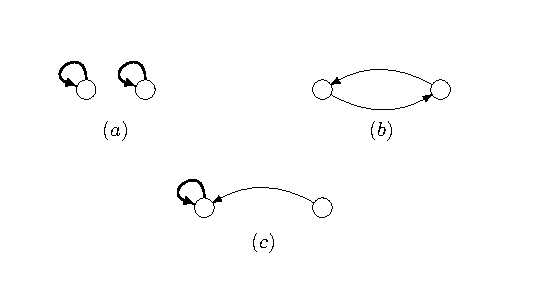
\includegraphics[scale=1.3]{figurenetworks.pdf}
\caption{Set of all possible networks with $N=2$ and $K=1$.}
\label{fig:rb}
\end{figure}

Topologies (a) and (b) have each the statistical weight $1/4$ in
the ensemble, since each of the links is connected in the
given way with probability $1/2$. Topology (c) has the
weight $1/2$, since there are two possibilities for realizing
this topology: either of the two nodes can be the one
with the self-link.


While the number of inputs of each node is fixed by
the parameter $K$, the number of outputs (i.e. of outgoing links) varies between the nodes. The mean number of
outputs must be $K$, since there must be in total the same
number of outputs as inputs. A given node becomes the
input of each of the N nodes with probability $\frac{K}{N}$ . In
the thermodynamic limit $N \to \infty$ the probability distribution of the number of outputs is therefore a Poisson
distribution:

$$
P_{out}(k) = \frac{K^k}{k!}e^{-K}
$$

\section{Dynamics}

All nodes are updated at the same time
according to the state of their inputs and to their update
function. Starting from some initial state, the network
performs a trajectory in state space and eventually arrives on an \emph{attractor}, where the same sequence of states
is periodically repeated. Since the update rule is deterministic, the same state must always be followed by the
same next state. If we represent the network states by
points in the $2^N$-dimensional state space, each of these
points has exactly one “output”, which is the successor
state. We thus obtain a graph in state space.
The size or length of an attractor is the number of
different states on the attractor. The basin of attraction
of an attractor is the set of all states that eventually
end up on this attractor, including the attractor states
themselves. The size of the basin of attraction is the
number of states belonging to it. The graph of states
in state space consists of unconnected components, each
of them being a basin of attraction and containing an
attractor, which is a loop in state space. The transient
states are those that do not lie on an attractor. They are
on trees leading to the attractors.


Let us illustrate these concepts by studying the small
$K = 1$ network shown in Figure~\ref{fig:rb2}, which consists of 4
nodes:

\begin{figure}[h]
\centering
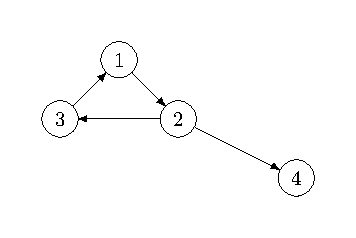
\includegraphics[scale=1.4]{figurenetworks2.pdf}
\caption{\emph{A small network with $N=4$ and $K=1$.}}
\label{fig:rb2}
\end{figure}

If we assign to the nodes 1,2,3,4 the functions invert,
invert, copy, copy, an initial state $1111$ evolves in the
following way:

$$
1111 \to 0011 \to 0100 \to 1111
$$

This is an attractor of period 3. If we interpret the bit se-
quence characterizing the state of the network as a number in binary notation, the sequence of states can also be
written as

$$
15 \to 3 \to 4 \to 15
$$

The entire state space is shown in Figure~\ref{fig:rb3}:
\begin{figure}[h]
\centering
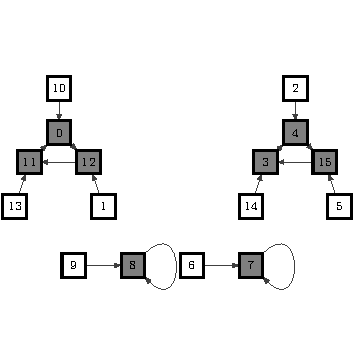
\includegraphics[scale=1.4]{fg3.pdf}
\caption{\emph{The state space of the network shown in Figure~\ref{fig:rb2}, if
the functions copy, copy, invert, invert are assigned to the four
nodes. The numbers in the squares represent states, and arrows indicate the successor of each state. States on attractors
are shaded.}}
\label{fig:rb3}
\end{figure}



There are 4 attractors, two of which are fixed points
(i.e., attractors of length $1$). The sizes of the basins of
attraction of the 4 attractors are $\Omega_1=6,\Omega_2= 6,\Omega_3 = 2,\Omega_4 = 2$. If the function
of node 1 is a constant function, fixing the value of the
node at 1, the state of this node fixes the rest of the
network, and there is only one attractor, which is a fixed
point.
\section{Phase transitions}
In RBNs, as well as in many dynamical systems, three
phases can be distinguished: \emph{ordered, chaotic, and critical} \cite{K19}.
These phases can be identified with different methods, since
they have several unique features.
these dynamical phases is related to
“sensitivity to initial conditions”, “damage spreading”, and
“robustness to perturbations” which are different ways of
measuring the stability of a network. We can “mutate”,
“damage” or “perturb” a node of a RBN by flipping its state.
We can also change a connection between two nodes, or in
the lookup table of a node. Since nodes affect other nodes,
we can measure how much a random change affects the rest
of the network. In other words, we can measure how the
damage spreads. This can be done by comparing the evolution of a “normal” network and a “perturbed” network. In
the ordered regime, usually the damage does not spread: a
“perturbed” network “returns” to the same path of the “normal” network. This is because changes cannot propagate
from one green island to another. In the chaotic phase, these
small changes tend to propagate through the network, making it highly sensitive to perturbations \cite{K49}.
An other feature is the convergence versus divergence of the
trajectories in state space of the network dynamics. In the ordered phase, similar states tend to converge to the same state.
In the chaotic regime, similar states tend to diverge. At the
edge of chaos, nearby states tend to lie on trajectories that
neither converge nor diverge in state space.
Living systems, or computing systems, need certain stability to survive, or to keep information; but also flexibility
to explore their space of possibilities. This has lead people
to argue that life and computation occur more naturally at
the edge of chaos or at the ordered regime
close to the edge of chaos \cite{K6}\cite{K49}.
\begin{figure}[h]
\centering
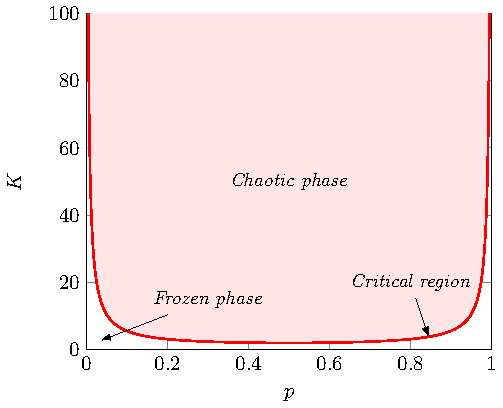
\includegraphics[scale=1.2]{images/phase-transition.pdf}
\caption{\emph{Phase diagram for the $N-K$ model. The shaded area corresponds
to the chaotic phase, whereas the white region corresponds to the chaotic phase.
The curve separating both regions is the critical phase.}}
\label{fig:ph-tr}
\end{figure}

Very early in the studies of
RBNs, people realized in simulations that the networks with
$K \le 2$ were in the ordered regime, and networks with $K \ge 3$,
were in the chaotic regime. In Figure \ref{fig:ph-tr} we can appreciate
characteristic dynamics of RBNs in different phases.
We can identify phase transitions in RBNs in different
ways. The main idea is to measure the effect of perturbations, the sensitivity to initial conditions, or damage spreading. This is analogous to Lyapunov exponents in continuous
dynamics.
The phase transitions can be statistically or analytically
obtained. Derrida and Pomeau were the first to determine
analytically that the critical phase (edge of chaos) was found
when $K = 2$ \cite{K8}\cite{K17}\cite{K21}.
following the model of Kauffman, RBN which most represent biological GRNs are those wich has $K=2$ \cite{K6}, because in the frozen phase (where $K=1$) networks are too simple to represent real regulatory networks; while in the caothic phase (where $K=3$) the time scales of the networks cycles grow exponentially, which is not biologically pheasible.
In Chapter \ref{analysis} we will see the differences in $K=1$ networks and $K=2$ networks.

\section{Attractor jumps}
In Kauffman model, attractors in the state space are considered as gene regulatory networks of different cells, where different attractors represent cells of different type, and where for example cancer cells lay in one specific attractor \cite{K3}\cite{K2}.
Now, if we suppose that different cell types lay in different attractors, we  suppose that the jump from an attractor to one other is given by a perturbation in the binary sequence of the genes.
So for example we take the previous network, and consider that we are in the state $12$ of the first attractor:
$$
12 \to 11 \to 0 \to 12
$$

And suddenly we change the state of the third node from $0$ to $1$:
$$
1100 \to 1110
$$

We change the system to have the state $14$ and so we jump into the second attractor:
$$
14 \to 3 \to 4 \to 15 \to 3
$$
\begin{figure}[h]
\centering
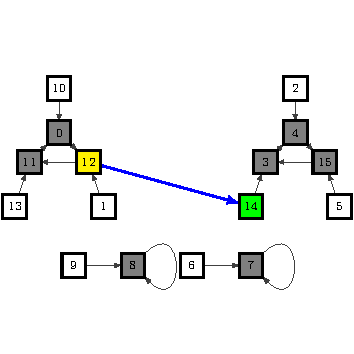
\includegraphics[scale=1.4]{fg4.pdf}
\caption{\emph{Jump from one attractor to one other in the state space.}}
\label{fig:rb4}
\end{figure}

So the branching pathways of differentiation between
attractors in a RBN in the ensembles create a directed
graph showing which attractors can be perturbed to reach which attractors.

In fact, if we consider all the possible stochastic perturbations in the binary sequence of the genes, we can get the all the possible transitions between the attractors, and what we obtain is an other network, where the nodes are the attractors and the frequencies of transitions can be used to build a random walk on this network\cite{K2}\cite{K3}\cite{K29}.



\chapter{Cancer attractors}
\lhead[\fancyplain{}{\bfseries\thepage}]{\fancyplain{}{\bfseries\rightmark}}

%\newcommand{\folder}{/path/to/folder}
\newenvironment{sistema}%
{\left\lbrace\begin{array}{@{}l@{}}}%
{\end{array}\right.}
In questo capitolo viene fatta una piccola introduzione al modello classico preda-predatore di Lotka-Volterra.
\section{The model}
We consider a physical system that can be described by an weighted interaction network among nodes that can assume different
dynamical states (in the case of a gene network the states $\sigma\in [0,1]$ and we have models similar to spin models).
In the simplest case, we introduce a stochastic dynamics using the probability $p_i(t)$ that the node $i$ is in the state $\sigma_i=1$
(then $1-p_i(t)$ is the probability to get $\sigma_i=0$) and we define a linear equation for the probability evolution
\begin{equation}
\dot p_i(t)=\sum_j \mathcal{P}_{ij}p_j(t)-\gamma_i p_i(t)
\label{average}
\end{equation}
where $\mathcal{P}_{ij}$ are transition probability rates and $\gamma_i^{-1}$ defines the mean lifetime of the excited state.
The meaning of the rates $\mathcal{P}_{ij}$ is the rate at which the excited state of the node $j$ increases (or decreases if
$\mathcal{P}_{ij}<0$) the probability of a transition to the excited state of the node $i$. Since $0\le p_i\le 1$ for all $i$, this space should be invariant for the dynamics. This condition depends on the spectral properties of the matrix
\begin{equation}
\mathcal{P}_{ij}-\gamma_j\delta_{ij}
\label{matrix}
\end{equation}
associated to the system. Let consider the case $\mathcal{L}_{ij}\ge 0$ (i.e. we have no inhibitory link),
the first quadrant is clearly invariant and if we define
$$
\sum_i  \mathcal{P}_{ij}=\hat \gamma_j>0
$$
the matrix 
$$
\mathcal{L}_{ij}=\mathcal{P}_{ij}-\hat \gamma_j \delta_{ij}
$$
is a Laplacian matrix and the system (\ref{average}) can be written in the form
$$
\dot p_i(t)=\sum_j \mathcal{L}_{ij}p_j(t)-\Delta \gamma_i p_i(t)\qquad \Delta \gamma_i=\gamma_i-\hat \gamma_i
$$
and by assumption we have $\gamma_i>\hat \gamma_i$. The eigenvalues of the matrix $\mathcal{L}_{ij}$
have all negative real part except the null eigenvalue. It follows that all the eigenvalue of the matrix (\ref{matrix})
has negative real part and the dynamics is a contraction towards the origin:
a stable solution (i.e. without any external stimulus the system relaxes to the $\sigma_i=0$ state).
A non trivial stationary can be achieved only if an external stimulus is inserted
\begin{equation}
\dot p_i(t)=\sum_j \mathcal{P}_{ij}p_j(t)-\gamma_i p_i(t)+\epsilon f_i(t)
\label{average_ext}
\end{equation}
The stationary solution has to satisfy $p_i\in [0,1]$ so that $f_i(t)\ge 0$ otherwise we can have negative probability 
when $p_i\simeq 0$. The case of a Laplacian matrix
$$
\hat \gamma_i=\gamma_i
$$
we get another possible stationary solution for $\mathcal{L}_{ij}p^\ast_j=0$ in the first quadrant and
the subspace $\sum p_i=0$ is invariant and the dynamics is a contraction in this subspace (in general).
Then the system a stable stationary solution even in absence of an external stimulus.\par\noindent
The presence of inhibitory links complicates the model and one has to prove that
\begin{itemize}
\item 1) there exists a physical space: an invariant cone in the first quadrant where the dynamics is a contraction towards
the origin;\par
\item 2) the external stimulus maintains the solution in the physical space.
\end{itemize}
Another solution could be to introduce boundary conditions so that $p_i\ge 0$ in any case (the system is non linear in such a case).
\par\noindent
The eigenvalues of the matrix (\ref{matrix}) define the different relaxation time scale the process and determine its rectivity
to the change of the external stimulus: in a typical problem one consider a slowly varying external stimulus so that the
system could be considered i a quasi stationary state
$$
\sum_j \mathcal{L}_{ij}p_j-\Delta \gamma_i p_i=-\epsilon f_i(t) \qquad \frac{df_i}{dt}\ll 1
$$
the derivative is small with respect to the eigenvalues of th matrix (adiabatic approximation). On the other hand we have the effect
of a correlated noise (we need to introduce a correlation in order have a continuous function $f_i(t)$). The problem is to
study the relation between the solution and the spectral properties of the matrix $\mathcal{L}_{ij}$: we simplify the
equation by assuming $\Delta \gamma_i=\Delta \gamma$ so that if $\lambda$ is an eigenvalue of $\mathcal{L}_{ij}$
then $\lambda-\Delta \gamma$ is an eigenvalue of the matrix (\ref{matrix}) and we assume that the dynamics
is perturbed by
\begin{equation}
\dot p_i(t)=\sum_j\left ( \mathcal{L}_{ij}+\Delta \mathcal{L}_{ij}\right ) p_j(t)-\Delta \gamma p_i(t)+\epsilon f_i(t)
\label{average_p}
\end{equation}
where the perturbation $\Delta\mathcal{L}_{ij}$ is a Laplacian matrix ($\sum_i \Delta\mathcal{L}_{ij}=0$ and we
assume $<\mathcal{L}>=0$) that can
represent an error in the measure of the transition rates $\mathcal{L}_{ij}$ or possible evolution of network due to
in time. In the first case we have an ensemble of transition matrices and we have to study the eigenvalue distribution
due to perturbation and the possible presence of bifurcation phenomena. In the second case we have a stochastic 
differential equation (since $\Delta \mathcal{L}_{ij}(t)$ can be represented as a realization of a stochastic process).
The possible approach are Perturbation Theory, Random Matrix Theory and Statistical Physics Methods for random matrices.
The external signal form the environment  (the environmental node) can be considered in the adiabatic approximation
(to be justified form a biological point of view).\par\noindent
The underlying stochastic process on the graph is defined by assigning the state $\xi_i(t)\in [0,1]$ at each node $i$ according 
to a probability distribution $\pi_i(t)$ that evolves as
$$
\dot \pi_i(t)=\sum_j \mathcal{L}_{ij}\xi_j(t)-\Delta \gamma \xi_i(t)+\epsilon f_i(t)
$$
By discretizing the dynamics for a time step $\Delta t$ we have the evolution
$$
\pi_i(t+\Delta t)=\pi(t)+\sum_j \mathcal{L}_{ij}\xi_j(t)\Delta t-\Delta \gamma \Delta t\xi_i(t)+\epsilon f_i(t)\Delta t
$$
and $\xi(t+\Delta t)$ realized according to the distribution $\pi_i(t+\Delta t)$ (stochastic cellular automata).
The average dynamics is computed by
\begin{eqnarray}
\dot <\pi_i(t)>&=&\sum_j \mathcal{L}_{ij}<\xi_j(t)>-\Delta \gamma <\xi_i(t)>+\epsilon f_i(t)\nonumber \\
&=&\sum_j \mathcal{L}_{ij}p_j(t)-\Delta \gamma p_i(t)+\epsilon f_i(t)=\dot p_i(t)\nonumber
\end{eqnarray}
and we recover the average equation (\ref{average}). But the stochastic dynamics gives information on the applicability
of the average approximation and the variability at the critical states (at bifurcation of the spectrum of $\mathcal{L}$).
The stochastic dynamics can be studied for stochastic connection matrices $\mathcal{L}+\Delta \mathcal{L}$.



%\documentclass[runningheads]{llncs}
%
%%\usepackage[latin9]{inputenc}
%%\usepackage{amsmath,amsthm}
%%\usepackage{braket}
%%\usepackage{amsfonts}

% Used for displaying a sample figure. If possible, figure files should
% be included in EPS format.
%
% If you use the hyperref package, please uncomment the following line
% to display URLs in blue roman font according to Springer's eBook style:
% \renewcommand\UrlFont{\color{blue}\rmfamily}
%
%
%\begin{document}
%
%\title{Stochastic models for dynamical systems on graphs and applications to genetic activity}
\chapter{The model}\label{model}
\lhead[\fancyplain{}{\bfseries\thepage}]{\fancyplain{}{\bfseries\rightmark}}
Models of boolean networks proposed by Kauffmann are limited and can't represent perfectly biological networks because of some considerations: simple RBNs present cahotic behaviours and attractors are not sufficient to explain cellular differentiation.
In this Chapter we present the theoretical model of GRNs based on RBNs.

\section{The underlying philosophy of the model}
The dynamical model is a schematic representation of the activity of gene regulatory networks introduced in Chapter \ref{grn}. We have to discuss the assumptions the define the model from a biological 
point of view: the main criticism to a model is that its assumptions cannot be justified by the biological mechanisms. 
Our goal is to model the genetic activity related to a differentiation process of a cell: i.e. this activity is a stable long term activity whose stability
is probably controlled by biochemical mechanisms (i.e. methylation processes), but for cancer cells the control dynamics is not so efficient allowing
the evolution of different cell populations. Then we assume that this evolution is possible due to the competition of different genetic activities through
dynamical mechanisms that can be triggered by the external environmental signals.
In particular we assume:
\begin{itemize}
\item the long term genetic activity is determined by the presence of small genetic networks that have a stable active dynamical state;
\item there exists an eternal control mechanism: the subnetworks have control nodes that prevent the arise of the active state in the subnetwork if there
are set to the inactive state;
\item once the active state has been established in a subnetwork it remains stable in time without any stimulus, except if an inhibitory stimulus 
change the state of control nodes;
\item the stability and the controllability properties of a subnetwork depends from the existence of loops in the subnetwork: a loop may be related to the activation
of metabolic cycles in the cell that define the cell behavior;
\item each node of a subnetwork may represent the state of a gene that is connected and regulates the activation of other genes;
\item in the cell differentiation mechanism is defined by the competition of different subnetworks that interact in a inhibitory way;
\item the mutation mechanism change the connectivity of the network: we may distinguish between permanent changes and dynamical change (i.e. a connection
may exist or non exist during time).
\end{itemize}
The complexity of the model is not a fundamental issue since we want to point out universal behaviors:  first of all the existence of bistability or bifurcation 
phenomena for simple model and the definition of control parameters.
%
\section{The mathematical model and related problems}
Here we studied the model dynamics in different situations using mathematical methods. The main idea is understand the dynamics of the models to point
out the universal properties that are robust and could explain the experimental data. The biological meaning of control parameters is a fundamental task
to apply the model to predict the results of new experiments.\par\noindent 
We consider a physical system that can be described by an weighted interaction network among nodes that can assume different
dynamical states (in the case of a gene network the states $\sigma\in \{0,1\}$ and we have models similar to spin models).
The interaction structure is defined by signed adjacency matrix $A_{ij}\in\{-1,0,1\}$ where the sign refers to a cooperative or antagonist interaction between the connected nodes. 
In the simplest case, we introduce a stochastic dynamics using the probability $p_i(\sigma, t)$ that the node $i$ is in the state 
$\sigma$ (we assume $\sigma>0$) at time $t$: in a deterministic approach $p_i(\sigma, t)=\delta(\sigma-\sigma(t))$
to denote that the node assume the state $\sigma=1$ with probability one. The evolution of a deterministic model
can be described by the equation
\begin{equation}
\sigma_i(t+1)=\Phi_i(\sigma(t))=\Theta\left (\sum_j A_{ij}\sigma_j(t)\right )
\label{evolnet}
\end{equation}
where $\Theta(x)\in[0,1]$ is a threshold sigmoidal function (we assume $A_{ii}=0$ to avoid self loops). \par\noindent
Remark: the dynamics is a information diffusion on the network. If we consider the linear system
$$
\zeta_i(t+1)=\sum_j A_{ij}\zeta_j(t)
$$
where $\zeta_i$ are non negative integers we have an equivalent dynamics since $\sigma_i=\Theta(\zeta_i)$ and it is possible
to study the linear system to derive some properties of the initial system. For example the relaxation time to the solution $\sigma_i=1$
$\forall\; i$ is for a given initial condition $\sigma^0_j=\delta_{jk}$ is $t=n$ such that the matrix $A^n$ has positive entries along the whole
$k$-th column. This mens that for each node $i$ there is a walk of length $n$ from the initial node $k$ to $i$.
\par\noindent
We also assume a cause-effect relation so that $A_{ij}$ is a directed
graph. The deterministic model is a Hopfield network (each node has at least an input and an output link; the environment nodes has only output links)
and one could study the equilibrium states and their stability. An equilibrium condition as follows is characterized as follows:
for each $i$ let
$$
Q_i(t)=\sum_j A_{ij}\sigma_j(t) 
$$
then $Q_i>0$ if $\sigma_i>0$ and vice versa.  Then $A_{ij}\ge 0$(i.e. $A_{ij}$ is a connectivity matrix for a directed network) 
implies that the non trivial equilibrium is $\sigma_i=1$: if $\sigma_k=0$ for some $k\in K$ then we have
$$
\sum_{j\notin K} A_{kj}\sigma_j=0
$$
so $A_{kj}=0$ for all $j\notin K$ and the network is disconnected. Then we have the trivial solution $\sigma_i=0$. For each equilibrium solution $\sigma^\ast$ we have a stability basin
$$
S_{\sigma^\ast}=\left \{\sigma \; | \; \lim_{t\to\infty} \sigma(t)=\sigma^\ast\right \}
$$
If $S_{\sigma^\ast}$ defined neighborhood of $\sigma^\ast$ the solution is stable or if $S_{\sigma^\ast}=\{\sigma^\ast\}$ the solution completely unstable. 
The stability of the origin depends on the existence of a Ljapounov function: let introduce the network activity
$$
\Sigma(t)=\sum_i \sigma_i(t)=\sum_i \Theta(Q_i(t-1))\ge \Sigma(t-1)
$$
since if each node has at least one input link, $A_{ij}=1$ implies $\sigma_j(t-1)\Rightarrow \sigma_i(t)=1$ and the activity cannot decrease. The solution $\sigma_i=0$
is completely unstable. If there would exists an equilibrium solution with $\sigma_k=0$ for some $k$ then we define $S_A$ the set of nodes s.t.
$$
i\in S_A\quad \Rightarrow \quad \sigma_i=0
$$
(obviously $\sigma_k\in S_A$). Let $S_{\bar A}$ the complement of $S_A$, the network dynamics implies
$$
0=\sum_j A_{ij}\sigma_j=\sum_{j\notin S_A} A_{ij}\sigma_j=0 \qquad \textrm{if}\quad i\in S_A
$$
so that $A_{ij}=0$ if $i\in S_A$ and $j\in S_{\bar A}$: i.e. there is not a cause-effect connection between $S_{\bar A}$ and $S_A$ and the state $\sigma_i=1$ for $i\in S_{\bar A}$
is an equilibrium state. Therefore we have as many equilibrium states as many partitions $S_A$ and $S_{\bar A}$ there exist such that $S_A$ triggers the activity of $S_{\bar A}$
but not vice versa. For any initial condition $\sigma_i(0)=\delta_{ik}$ the possible evolution are a periodic orbit or an equilibrium state: one can detect all the equilibrium conditions
by $\sigma^\ast$ by the condition
$$
\sigma_i^\ast=1\quad \textrm{if}\quad \sigma_i(t)=1\quad \textrm{for}\;\textrm{some}\quad t\ge 0
$$
The equilibrium states are a semigroup: let $\sigma^a$ and $\sigma^b$ two equilibrium states the
$$
\sigma^a\cup \sigma^b=\sigma^c
$$
is still an equilibrium. An example: if there exit a one directional loop $\gamma$ in the network and there is no output link
from $\gamma$ to the remaining nodes of the network then $\sigma_i=1$ for any $i\in \gamma$ is an equilibrium.
If the loop is simple (each node has a one input link and one output link) the equilibrium is neutral since any change
$\sigma_i=1\to\sigma_i=0$ creates a periodic orbit (the total activity is constant). But if we we add a link to the loop
then we get a stable solution since a single node can trigger the activity of two nodes and the equilibrium is an attractive
stationary state (see figure \label{fig:onecluster}). If a node is accidentally set to zero this anomaly propagates in the loop, 
until it reaches the node $4$ where it is annihilated by the activity of the node $(2)$. The average lifetime of a single perturbation
is the average path length to propagate to the node $(4)$ from the initial node (therefore it depends from the loop length or in case
of presence of many loops, the average path length is computed considering independent loops). 
\vskip .5 truecm 
\begin{figure}
\begin{center}
\begin{tikzpicture}
[->,>=stealth',shorten >=1pt,auto,node distance=3cm,
                    thick,main node/.style={circle,draw,font=\Large}]

  \node[main node] (1) {1};
  \node[main node] (2) [below left of=1] {2};
  \node[main node] (3) [below right of=2] {3};
  \node[main node] (4) [below right of=1] {4};

  \path[every node/.style={font=\small}]
    (1) edge node [left] {+1} (4)
    (2) edge node [right] {+1} (1)
        edge node {+1} (4)   
    (3) edge node [right] {+1} (2)
    (4) edge node [left] {+1} (3);
    \label{schema1}
\end{tikzpicture}
\end{center}
\caption{\emph{Example of random boolean network.}}
\label{fig:onecluster}
\end{figure}
\vskip .5 truecm
The boolean network models the propagation of information. By studying the stability problem of the solution $\sigma_i=1$ it is convenient to introduce the dual dynamics:
$$
\sigma_i^c(t+1)=\Theta\left (\prod_{j\sim i} A_{ij}\sigma^c_j(t)\right )=\prod_{j\sim i} A_{ij}\sigma^c_j(t)
$$
where $\sigma_i^c=1-\sigma_i$ is the dual state of the node and the product is restricted to the nodes connected to $i$
($A_{ij}\ne 0$): i.e. the node $(4)$ takes the state $\sigma^c=1$ only if both the nodes
$(1)$ and $(2)$ in that state at previous time. This dynamics is valid for any configuration of the network and the state $\sigma^c=1$
moves on the network until it reaches an absorbing state for which
$$
\prod_{j\sim i} \sigma^c_j(t)=0 \quad \forall \; i
$$
For a given stable equilibrium $\sigma^\gamma$ state associated to a loop $\gamma$ any environmental perturbation
that set to zero a activity of a node will destroy the equilibrium after a time equal to the number of the loop nodes minus one.
For example in the figure there are two loops $((1)\to (2)\to (3)\to (4))$ and $((2)\to(4)\to (3))$ if we set to zero the node 
$(4)$ after three iterations all the nodes will be in the zero state. The two loops are nit independent since one loops contains the other). On the contrary if we set to zero the node $(1)$ one loop remains active. This remark allows to introduce the concept of control node: a node is a control node if its state is able to 
force the state of the whole network. The effect of a thermal bath could be introduced by assuming that the state of a node
is defined as random variable that takes value $\sigma_i(t)=1$ with probability $p_i(t)$ where 
\begin{equation}
p_i(t+1)=\Theta_T\left (\sum_j A_{ij}\sigma_j(t)\right )
\label{stocdyn}
\end{equation}
and $\Theta_T(x)$ is a logistic function 
$$
\Theta_T(x)=\frac{1}{2}\left (1+\textrm{tgh}(x/T-\epsilon)\right )
$$
where $\epsilon$ measures to tendency of the network to be in the idle state when no stimulus is present.
The logistic function is a generic sigmoidal function we do not expect that the specific form of $\Theta_T(x)$ is critical for the results.
\par\noindent



Remark: since the values of $x$ are
quantized to integer in any case, if $\epsilon>T^{-1}$ the idle state is statistically attractive so $\epsilon$ could define a critical temperature
for the network activation. We recover the deterministic dynamics for $T\to 0$. As a stochastic process we have a Markov process (since
the realization of the variable $\sigma_i(t+1)$ depends only on the present state $\sigma_j(t)$ of the network. The dynamics (\ref{stocdyn})
is a Markov field: the realization of the variable $\sigma_i$ depends only from the present state of the network (and not from past states) and
only from the states of the connected nodes $A_{ij}\ne 0$. The last condition (Markov field) means that the realizations of $\sigma_i(t)$
and $\sigma_j(t-1)$ are independent if the nodes are not connected. The transition probabilities depend from the state of the network
and one derives the average dynamics
\begin{equation}
<\sigma_i>(t+1)=p_i(t+1)=\left \langle \Theta_T\left (\sum_j A_{ij}\sigma_j(t)\right ) \right \rangle\simeq
 \Theta_T\left (\sum_j A_{ij}p_j(t)\right ) 
\label{avestoc}
\end{equation}
Then we have two possibilities: if the total average network activity tends to increase
\begin{equation}
\bar \Sigma(t+1)=\sum_i p_i(t+1) =\sum_i  \Theta_T\left (\sum_j A_{ij}p_j(t)\right ) > \bar \Sigma(t)
\label{condave}
\end{equation}
the equilibrium solution $\sigma_i=1$ is attractive, on the contrary we have a an average tendency to decrease the network activity. 
The situation is illustrated in the fig. \label{fig:crit}
\begin{figure}[h]
\label{fig:crit} 
\centering{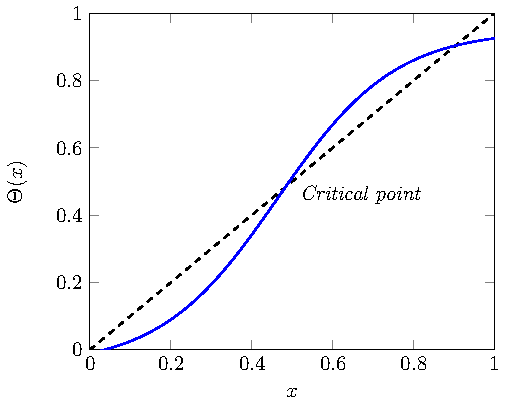
\includegraphics[scale=1.3]{images/theta.pdf}}
\caption{\emph{Possible behavior for the condition (\ref{condave}); the units are arbitrary and scale with the network dimension.}}
\end{figure}
Remark: the mean field approximation apply when the $\Theta_T(x)$ can be approximated by a linear function locally: i.e. the fluctuations are small
enough to approximate the function by a linear function in the whole fluctuation range. This is certainly not true when we have fat tail fluctuations.
\par\noindent
Except for a small initial region, the condition (\ref{condave}) can be satisfied up to a critical value of the network activity $\Sigma$ (if the temperature
is not too big), so that the average activity tends to increase. But if the activity is below the critical value then the network activity tend to decrease and
the stability of the solution $\sigma_i=1$ is lost. A connected network tends to be more stable since the quantities
$\sum_j A_{ij}\sigma_j$ increase.  This picture is clearly an approximation since we neglect the fluctuation effects: if the fluctuations are big (this
depends also on the connectivity matrix) we may have a fast transition between the two possible regime and a correction of the critical value. The
critical vale is a consequence of the sigmoidal behavior of the $\Theta_T(x)$ function and its depends on the temperature and on the $\epsilon$
values. In presence of fluctuations and of two dynamical regimes (active and non active) we expect that the network activity may switch from one regime
to another with a characteristic time scale (Kramer transition rate Theory, see Chapter \ref{kramer}). The transition may be triggered by large fluctuations that are both consequence
of rare events (in such a case the probability should be exponentially small with respect the activity) but also depend on the network structure (the presence of
hub nodes that can change the activity of many nodes amplifies the effect of small fluctuations (i.e. the change of the hub node state) and may introduce
fat tail statistic in the fluctuation distribution). A second stochastic effect is related to the fluctuations of the connectivity due to environmental causes: 
the matrix $A_ij(t)$ is a stochastic process (so that its entries change their value according to a probability distribution). The simplest model can be formulated as
follows: we assume that the nonzero entries $A_{ij}(t)$ assume value $1$ with a given probability $p$ (independent from the network state)
 each time step $\Delta t$ (i.e. we are not simulating
a parametric white noise, but a correlated random noise with a define correlation time scale $\Delta t$). $\Delta t$ is the shortest evolution time scale
for the system (we need a physical interpretation) and we set $\Delta t=1$. The effect of a parametric noise is substantially different from the environmental noise
and the evolution equation (\ref{evolnet}) reads
\begin{equation}
\sigma_i(t+1)=\Theta\left (\sum_j A_{ij}(t)\sigma_j(t)\right )
\label{evolnetstoc}
\end{equation}
In such a case the average dynamics is not useful and the problem can be studied by the representative dynamics
$$
\zeta_i(t+1)=\sum_j A_{ij}(t)\zeta_j(t)\qquad \Rightarrow \qquad \zeta(t)=\prod_{k=1}^t A(k)\zeta(0)
$$
where the solution is the product of random matrices (there are results on the spectral properties). From a biological point of view means
that the interaction of genes depends also by external factors. \par\noindent  
One could say that the network is active if a certain condition is satisfied (for example the average
total activity should overcome a given threshold) so that fluctuation may introduce the existence of non active states.
Problems for a single network: starting from a loops with a fixed dimension adds randomly links to stabilize the
equilibrium solutions (existence of sub-loops)  and study the robustness of the solution and the recovery times in relation with
the connectivity matrix; adding the temperature, study the existence of critical value for the appearance of the equilibrium solution; the thermodynamic limit. The effect of the environmental noise has to be justified from a biological point of view by relating it
to the individual variability of the cell phenotypes in an homogeneous population.\par\noindent
In the stochastic models one should also consider the problem that the connectivity matrix is not fixed (for example we have
a ensemble of admissible matrices or the existence of the links is a random event). In such a case we have a stochastic
dynamics
\begin{equation}
\sigma_i(t+1)=\Theta\left (\sum_j A_{ij}(t)\sigma_j(t)\right )
\label{stocdyn2}
\end{equation}
where $A_{ij}(t)$ is a random process with value $\in\{0,1\}$ maintaining some average properties of the connectivity;
this is an alternative to the environmental noise (parametric noise). This model simulates the fact that the activation of a link
may depends on random events (i.e. not only from the existence of the link) so that a genetic network is indeed a stochastic
network. In principle any realization of the connectivity matrix $A_{ij}$ has an equilibrium $\sigma_i=1$ but the robustness
of equilibrium can be influenced by the fluctuations. Problem: if the robustness of the equilibrium with respect to the external
perturbations (i.e. an external signal on a node) depends on the spectral properties of the connectivity matrix then
it is possible to study the spectral properties of random connectivity matrices and develop a control theory
for the network. 
\par\noindent
Let us consider the existence of competitive networks (see Figure \ref{fig:comp}) that are linked by inhibitory links: if the first network is
in an exited state the second network should be completely switched off for a stable equilibrium.
\vskip .5 truecm

\begin{figure}
\centering
\begin{tikzpicture}[->,>=stealth',shorten >=1pt,auto,node distance=2.5cm,
                    thick,main node/.style={circle,draw,font=\Large}]

  \node[main node] (1) {1};
  \node[main node] (2) [below left of=1] {2};
  \node[main node] (3) [below right of=2] {3};
  \node[main node] (4) [below right of=1] {4};
  \node[main node] (5) [right of=4] {5}; 
  \node[main node] (6) [below right of=5] {6};
  \node[main node] (7) [above right of=6] {7};
  \node[main node] (8) [above left of=7] {8};

\path[every node/.style={font=\small}]
    (1) edge node [left] {+1} (4)
         edge[red] node [red] {-1} (8)
    (2) edge node [right] {+1} (1)
         edge node {+1} (4)   
    (3) edge node [right] {+1} (2)
    (4) edge node [left] {+1} (3)
    (8) edge node [left] {+1} (7)
    (5) edge node [right] {+1} (8) 
    (6) edge node [right] {+1} (5)
        edge[red] node [red] {-1} (3)
    (7) edge node [left] {+1} (6)
            edge node {+1} (5)  ;
\end{tikzpicture}
\caption{\emph{Example of a network composed by two competitive subnetworks.}}
\label{fig:comp}
\end{figure}
\par\noindent
If we start with all the node states set to one we create a frustrated situation, otherwise the network choose one
of the two possible stable states. In such a case the presence of an environmental noise could induce the transition
to one state to another (to be studied). An external forcing breaks the symmetry.\par\noindent
We expect a transition phase as a function of the temperature: increasing the temperature the node states tends 
to be independent, but under a threshold the system should choose a stationary state. 
\par\noindent
The system can be generalized to consider the interactions of different cooperative networks (possibly with different internal
structure) that are connected by inhibitory links (in the case of connection with excitatory links we join the subnetwork in a 
single one). We can introduce a metadynamics where $\nu_k(t)$ is the state of the $k$ subnetwork and
we have a relation
\begin{equation}
\nu_k(t+\Delta t)-\nu_k(t)=\phi(\nu_k(t))-\gamma\left (H_{kj}\nu_j(t)\right )
\label{metastoc}
\end{equation}
where $H_{hk}\ge 0$ is an inhibitory connectivity matrix. $\phi(\nu_k(t))$ describes the tendency of the sub-network to increase
its activity and $\gamma$ the average decreasing of the activity due to the presence of other sub-networks.
This is an effective equation: $\nu_k$ should describe the network activity (i.e. it could be the time-average activity of the nodes
assuming that the network could be considered in a stationary state). Indeed the evolution time scale $\Delta t$ could be assumed
$\Delta t\gg 1$ so that the subnetwork states are relaxed to a stationary states. 
The structure of attraction basins of the stable states could be related to a potential in the state space if
$$
\nu_k(t+1)-\nu_k(t)=-\frac{\partial }{\partial \nu_k}\left [ \frac{\gamma}{2} \sum_{ij}\nu_i H_{ij}\nu_j+\sum_j V(\nu_j)\right ]
$$
where 
$$
\phi(\nu)=-\frac{\partial V}{\partial \nu}
$$
Since $\phi(\nu)\ge 0$ $V(\nu)$ is increasing. Then we introduce the energy
$$
E=\frac{\gamma}{2} \sum_{ij}\nu_i H_{ij}\nu_j+\sum_j V(\nu_j)
$$
and the equilibrium are the critical points of the energy. Moreover 
\begin{eqnarray}
E(t+1)-E(t)&\simeq& (\nu_k(t+1)-\nu_k(t))\frac{\partial}{\partial \nu_k}\left [\frac{\gamma}{2} \sum_{ij}\nu_i(t) H_{ij}\nu_j(t)+\sum_j V(\nu_j(t))\right ]\nonumber \\
&=& -\frac{1}{2}\frac{\partial}{\partial \nu_k}\left [ \frac{\gamma}{2} \sum_{ij}\nu_i(t) H_{ij}\nu_j(t)+\sum_j V(\nu_j(t)) \right ]^2\nonumber
\end{eqnarray}
Therefore the energy is a Ljapounov function and the system equilibria are defined by the critical points of the Energy function
corresponding to local minima and maxima.\par\noindent
Remark: the existence of the Energy implies that $H_{ij}$ is symmetric negative defined
$$
\frac{\partial^2 E}{\partial \nu_j \partial \nu_i}=\frac{\partial^2 E}{\partial \nu_i \partial \nu_j}
$$
\par\noindent
The stochastic effect has to be introduce but it is possible a thermodynamics approach and a thermodynamics equilibrium exists
according to the Maxwell-Boltzmann distribution and the detailed balance condition. This means that the whole network does not
satisfy this condition, but the metadynamic network realized a reversible Markov process. The existence of a thermodynamic equilibrium
allows to use Maximal Entropy Principle and the Maxwell Boltzmann distribution when we introduce a thermal bath. 
\par\noindent
We are interested in networks with many different equilibria each one related to exited state of subnetworks (or a combination of subnetworks), 
in the effect of a thermal noise and in the effect of external forcing. The external  we introduce in the network boundary nodes whose state is defined by a given external signal
$\sigma_b(t)$ (possible a stochastic process) then the network dynamics reads
$$
\sigma_i(t+1)=\Theta\left (\sum_j A_{ij}\sigma_j(t)+\sum_b A_{ib}\sigma_b(t)\right )
$$
where $A_{ib}$ is the link between the environmental node $b$ and the node $i$. It is possible to introduce a probabilistic description of the evolution
of the probability that the network is in the state $\sigma'$ at time $t+1$ according to
\begin{equation}
p(\sigma',t+1)=\sum_{\sigma}\pi(\sigma',\sigma)p(\sigma,t)
\label{lapla}
\end{equation}
where
$$
\pi(\sigma'|\sigma)=E\left (\delta_{\sigma',\Phi_{\sigma_b}(\sigma)} \right )
$$
and the expectation value is computed on the realization of the input noise. $\pi(\sigma'|\sigma)$ is the transition rate per unit time (the continuous limit could be considered).
Let $\sigma_{eq}$ stable equilibrium state the effect of external random perturbations could be to move the network state in a neighborhood of the equilibrium solution
or it could induce a transition to other equilibrium basin attractions so that the dynamics starts to perform an intermittence behavior. In such a case the relevant quantities are  
the residence times in the different basins that can be associated to metastable states.
\par\noindent
We introduce the stochasticity in the system assuming that the adjacency matrix is not known: i.e. $A_{ij}$ is a extracted from an ensemble of random matrices.
As the result of an experimental one could assume that each entry $A_{ij}$ is a dichotomous random variable with probability $p_{ij}$ to get the value $\pm 1$ (i.e. the
link is active). The value $p_{ij}=0$ is admitted so that the corresponding link it always inactive. The problems are:
\begin{enumerate}
    	\item Classifying the equilibrium states in relation to their robustness with respect the changes in the adjacency matrix;
     \item Understanding the representativity of the average dynamics: i.e. substituting the adjacency matrix with an average matrix one highlights the dynamical properties 
     that are correctly described by the average system
     \item Pointing out the existence of bifurcation phenomena so that it is possible to divide the ensemble in different communities with similar dynamical behaviors.
\end{enumerate}


\chapter{Analysis}\label{analysis}
\lhead[\fancyplain{}{\bfseries\thepage}]{\fancyplain{}{\bfseries\rightmark}}

In this Chapter we explain the starting implementation and analysis of the model following biological considerations.

\section{Implementation}

The theoretical model has been analyzed making simulations using Python.
The first thing was to create a class \emph{Random Network} to have a random boolean graph as an object, with its nodes and links, represented by a boolean adjacency matrix.

Every random network is a directed graph and is built to avoid self-loops, this means to create a random, boolean, and non-symmetric adjacency matrix with null trace.

The first thing to evaluate was to choose the average number of incoming links for each RBN. In Figure \ref{fig:K} we can see that the average discrete evolution of $100$ different realizations of RBNs, with increasing size.
\begin{figure}[h]
\centering
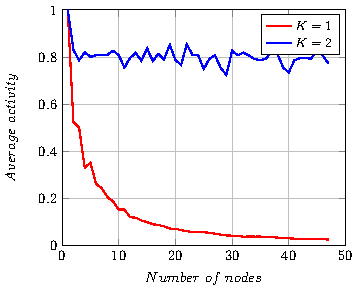
\includegraphics[scale=1.5]{images/K.pdf}
\caption{\emph{Plot of the average activity of the nodes with network of increasing size.
In the case of $K=1$ (i.e. the average number of incoming link for each network is one), the average activity decreases exponentially with the size of the network; in the case of $K=2$ instead, the average activity of the nodes remains stable with the network size.}}
\label{fig:K}
\end{figure}
In the case of $K=1$, i.e. the average number of incoming links for each network is one, the average activity decreases exponentially with the size of the network; in the case of $K=2$ instead, the average activity of the nodes remains stable with networks of increasing size. Moreover, network with only one incoming link means that the network is composed by only one big loop, which is unstable against envinromental noise. Instead, we look for networks which are stable in their state but also can be perturbed by noise. For this reason, the network considered for this model will take the parameter K constant: $K=2$.
Moreover, we can analyze the average number of outgoing links depending on the network size: In Figure \ref{fig:outgoing}, we can see that the average number of outgoing links tends to the parameter $K$.
\begin{figure}[h]
\centering
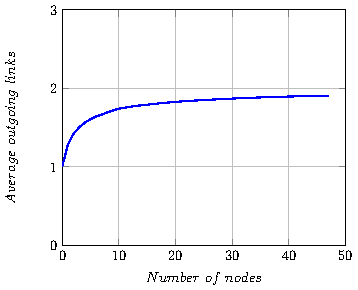
\includegraphics[scale=1.5]{images/outgoing.pdf}
\caption{\emph{Plot of the number of the outgoing links depending on the network size. We can see that the average tends to the parameter $K$. }}
\label{fig:outgoing}
\end{figure}




\section{Discrete evolution}
As shown in Chapter \ref{model}, the discrete time evolution of the network is given by the equation:
$$
\mathnormal{\sigma_i(t+1)=\Theta\biggl(\sum_jA_{ij}\sigma_j(t)\biggr)}
$$
where $A$ is the connectivity matrix of the network.
So this means that each node which has at least one incoming link with a node which is active, in the next step this node will be active.
At each time step we can measure the average activity of the network, which is the average number of nodes with the value:
$$
\sigma_i(t) = 1
$$


\section{Loops and Control nodes}
In simple random networks one can always find the number of independent loops.
Independent loops determine the complexity of the networks\cite{K38}, and are important for the construction of the model. In fact from the independent loops one can find the \emph{control nodes} of the network, which are the nodes that theirstate are able to force the state of the whole network, and are the nodes with maximum connectivity. Control nodes determine the whole activity and stability of the network. 
In RBNs with parameter $K=2$, we can see in Figure \ref{fig:loops} that the number of independent loops is linear with the network size.
\begin{figure}[h]
\centering
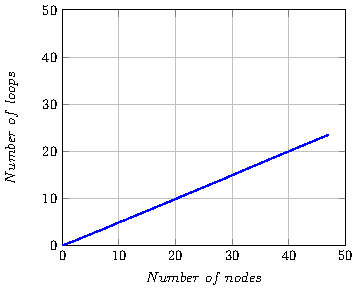
\includegraphics[scale=1.5]{images/loops.pdf}
\caption{\emph{Plot of the number of independet loops in the networks depending on the network size.}}
\label{fig:loops}
\end{figure}



\section{Noise}
The second thing to evaluate is the effect of the noise on the evolution of the network and the difference between noise and parametric noise, where parametric noise refers to the noise which infers in the links and not on the nodes.
To add noise to the system, during the discrete evolution of the network, at each time step there is a probability $p$ for the node or for the link to be turned off.
In Figure \ref{fig:noise} we can see the behavior of the average activity of the network depending on the amount of noise added. The plot is similar to a sigmoidal functions in both of the cases. In the case of noise added to the links the average activity results to be bigger than the case of noise added to the nodes. This is reasonable in the sense that since the number of links is less than the number of nodes so the effect of the noise among the links is less.
\begin{figure}[h]
\centering
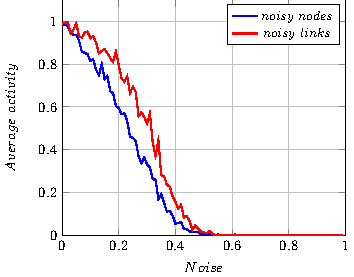
\includegraphics[scale=1.5]{images/noise.pdf}
\caption{\emph{Plot of the effect of the noise on the average activity on the network. In blue the noise works on the nodes on the network, while in red the noise works on the links. Number of nodes for each network: 10; Number of realizations for each value of noise: 100; }}
\label{fig:noise}
\end{figure}


\chapter*{Conclusions}
\lhead[\fancyplain{}{\bfseries\thepage}]{\fancyplain{}{\bfseries\rightmark}}

In this work we proposed a theoretical model for cell differentiation.
Since this biological process is governed by Gene Regulatory Networks, this networks can be modelled by Random Boolean Networks, in which each gene can be represented by  node which can be "on" or "off".
The process of differentiation is a multistable dynamical system, and involves different type of cells, but all of these start from one unique type of cell: the stem cells. The complexity of this process lays in the fact that cells "can" decide if transforming in one type of cell with respect one other, and for this reason seems phesible that if a network for a type of cell is active, it may hinibit the network for a different type of cell.
This process concerns also the birth of cancer cells: cancers cell can be governed by a specific type of regulatory network, which often is inactive, but due to some envinromental noise and stimuli it can be activated and gives an irreversible process of production of cancer cells. This can be seen as a local minima of the Waddington potential, which is impossible to escape.
The role of noise in this model is crucial, but it is well known that biological process are indeed very dependent to external noise.
Today, constructing Gene Regulatory Networks from sequencing data is still impossible, so future studies on Random Boolean Networks may give a way on a deeper understanding of these. 


\begin{thebibliography}{90}             %crea l'ambiente bibliografia
\rhead[\fancyplain{}{\bfseries \leftmark}]{\fancyplain{}{\bfseries
\thepage}}
%%%%%%%%%%%%%%%%%%%%%%%%%%%%%%%%%%%%%%%%%aggiunge la voce Bibliografia
                                        %   nell'indice
\addcontentsline{toc}{chapter}{Bibliography}
%%%%%%%%%%%%%%%%%%%%%%%%%%%%%%%%%%%%%%%%%provare anche questo comando:
%%%%%%%%%%%\addcontentsline{toc}{chapter}{\numberline{}{Bibliografia}}

\bibitem{K13} Waddington CH, \emph{The strategy of the genes: a discussion of some aspects of theoretical biology}. London: Allen and Unwin, (1957)
\bibitem{K10} Cameron P. Gallivan, Honglei Ren and Elizabeth L. Read,\emph{Analysis of Single-Cell Gene Pair
Coexpression Landscapes by
Stochastic Kinetic Modeling Reveals
Gene-Pair Interactions in
Development},doi: 10.3389/fgene.2019.01387 ,(2019)

\bibitem{K11} Jifan Shi, Tiejun Li , Luonan Chen, Kazuyuki Aihara,\emph{Quantifying pluripotency landscape of cell
differentiation from scRNA-seq data by
continuous birth-death process},https://doi.org/10.1371/journal.
pcbi.1007488 ,(2019)
\bibitem{K12} Jin Wang, Kun Zhang, Li Xu, and Erkang Wang ,\emph{Quantifying the Waddington landscape and biological
paths for development and differentiation}, https://doi.org/10.1073/pnas.1017017108 ,(2011)

\bibitem{K4} S. Huang, I. Ernberg, S. Kauffman,\emph{Cancer attractors: A systems view of tumors from a gene network
dynamics and developmental perspective}, doi:10.1016/j.semcdb.2009.07.003, (2009)
\bibitem{K1} S. A. Kauffman, \emph{Metabolic Stability and Epigenesis in
Randomly Constructed Genetic Nets}, J. Theoret. Biol. (1969)
\bibitem{K5} Drossel B.,\emph{Random Boolean Networks},arXiv:0706.3351 ,(2008)
\bibitem{K3} R.Serra, M. Villani, A. Barbieri, S.A. Kauffman, A. Colacci,\emph{On the dynamics of random Boolean networks subject to noise:
Attractors, ergodic sets and cell types.},J Theor Biol 265: 185–193, (2010)
\bibitem{K2} M. Villani, A. Barbieri, R. Serra,\emph{A Dynamical Model of Genetic Networks for Cell Differentiation}, doi:10.1371/journal.pone.0017703.g001,(2011)
\bibitem{K9} M. Ali Al-Radhawi , Nithin S. Kumar, Eduardo D. Sontag , Domitilla Del Vecchio, \emph{Stochastic multistationarity in a model of the hematopoietic
stem cell differentiation network},doi:10.1109/cdc.2018.8619300, (2018)
\bibitem{K39} Janeway, \emph{Immunobiology}, 9th Edition
\bibitem{K40} E. Davidson, M. Levine, \emph{Gene Regulatory Networks}, doi:10.1073/pnas.0502024102, (2005)
\bibitem{K37} Chen L et al., \emph{Biomolecular networks: methods and applications in systems biology}, Wiley, Hoboken ,(2009)
\bibitem{K43} Peccoud, J. and Ycart, B., \emph{Markovian Modelling of Gene Products Synthesis.}, https://doi.org/10.1006/tpbi.1995.1027, (1995)
\bibitem{K44} T.B. Kepler and T.C. Elston, \emph{Stochasticity in transcriptional regulation: origins, consequences, and mathematical representations}, 10.1016/S0006-3495(01)75949-8 , (2001)
\bibitem{K45} J.M. Pedraza, J. Paulsson, \emph{Effects of molecular memory and bursting on fluctuations in gene expression}, 10.1126/science.1144331, (2008).
\bibitem{K46} Y. Sasai \emph{Cytosystems dynamics in self-organization of tissue architecture}, https://doi.org/10.1038/nature11859, (2013)
\bibitem{K47} B. Zhang and P. G. Wolynes, \emph{Stem cell differentiation as a many-body problem}, https://doi.org/10.1073/pnas.1408561111, (2014)
\bibitem{K48} Zhou et al., \emph{Fast Pyrolysis of Glucose-Based Carbohydrates withAdded NaCl Part 2: Validation and Evaluation of theMechanistic Model},DOI 10.1002/aic.15107, (2016)
\bibitem{K41} A. Wuensche, \emph{Genomic regulation modeled as a network with basins of attraction}, Pacific Symposium on Biocomputing. Pacific Symposium on Biocomputing, (1998)
\bibitem{K49} S. A. Kauffman, \emph{Investigations}, Oxford University
Press, (2000)
\bibitem{K42} MacArthur S. et al., \emph{Developmental roles of 21 Drosophila transcription factors are determined by quantitative differences in binding to an overlapping set of thousands of genomic regions},doi:10.1186/gb-2009-10-7-r80 (2009)
\bibitem{K7} S. A. Kauffman: J. Theor. Biol., 44, Physica D, 10, 145 (1984)
\bibitem{K6} S. Kauffman, \emph{A proposal for using the ensemble approach to understand
genetic regulatory networks},Journal of Theoretical Biology 230 (2004) 581–590 ,(2004)
\bibitem{K8} B. Derrida, \emph{Random Networks of Automata: A Simple Annealed
Approximat ion.}, (1985)
\bibitem{K17} B. Derrida and H.Flyvbjerg, \emph{The random map model: a disordere model with deterministic dynamics}, J.Physique, (1987)
\bibitem{K21} B. Derrida, \emph{Spin glasses, random boolean networks and simple models of evolution}

\bibitem{K50} C.W. Gardiner, \emph{Handbook of Stochastic Methods}, Springer, (1985)
\bibitem{K26} Sui Huang , Ingemar Ernberg, and Stuart Kauffman,\emph{Cancer attractors: A systems view of tumors from a gene network
dynamics and developmental perspective}, DOI:10.1016/j.semcdb.2009.07.003, (2009)














\bibitem{K15} M. Rybarsch and S. Bornholdt,\emph{On the dangers of Boolean networks:
Activity dependent criticality and threshold networks not faithful to biology}, arXiv:1012.3287v1. (2010)
\bibitem{K16} J. Park and M. E. J. Newman,\emph{The statistical mechanics of networks}, DOI: 10.1103/PhysRevE.70.066117 (2004)
\bibitem{K17} C. Gershenso,\emph{Introduction to Random Boolean Networks}, arXiv:nlin/0408006,(2004)

\bibitem{K19} R. V. Solè, B. Loque, \emph{Phase transitions and antichaos in generalized Kauffman networks},Physics Letters,(1994)
\bibitem{K20} J. T. Lizier, S. Pritam, M. Prokopenko, \emph{Information dynamics in small-world Boolean networks}, (2011)

\bibitem{K22} A. Rèka and A-L. Barabàsi, \emph{Statistical mechanics of complex networks}, Reviewes of modern physics, Volume 74,(2002)
\bibitem{K23} N. Masuda , M. A. Porter, R. Lambiotte ,\emph{Random walks and diffusion on networks},Physics Reports 716–717 1–58,(2017)
\bibitem{K24} T. Biyikoglu, J. Leydold, P. F. Stadler,\emph{Laplacian Eigenvectors of Graphs}, Springer
\bibitem{K25} Fan R. K. Chung,\emph{Spectral Graph Theory}, CBMS

\bibitem{K27} M. Ali Al-Radhawi, Nithin S. Kumar, Eduardo D. Sontag, Domitilla Del Vecchio ,\emph{Stochastic multistationarity in a model of the hematopoietic
stem cell differentiation network},DOI:10.1109/cdc.2018.8619300.,(2018)
\bibitem{K28} Rushina Shah, Domitilla Del Vecchio,\emph{Reprogramming cooperative monotone dynamical systems},DOI:10.1109/cdc.2018.8618649, (2018)
\bibitem{K29} Atefeh Taherian Fard and Mark A. Ragan, \emph{Modeling the Attractor Landscape of
Disease Progression: a
Network-Based Approach},DOI: 10.3389/fgene.2017.00048, (2017)
\bibitem{K30} Sui Huang, Yan-Ping Guo, Gillian May, Tariq Enver,\emph{Bifurcation dynamics in lineage-commitment in bipotent progenitor cells},Developmental Biology 305, (2007)
\bibitem{K31} Xin-She Yang and Young Z. L. Yang,\emph{Cellular Automata Networks},arXiv:1003.4958 , (2010)

\bibitem{K34} Xin Kang, Chunhe Li,\emph{Landscape inferred from gene expression data governs pluripotency in
embryonic stem cells},Computational and Structural Biotechnology Journal 18 (2020) 366–374,(2020)
\bibitem{K35} Genaro J. Martinez , Andrew Adamatzky  ,
Bo Chen , Fangyue Chen , Juan C.S.T. Mora ,\emph{Simple networks on complex cellular automata:
From de Bruijn diagrams to jump-graphs},(2017)



\bibitem{K38} Schnakenberg J., \emph{Network theory of microscopic and macroscopic behavior of master equation systems.}, Reviews of Modern Physics,Vol.48, (1976)



\end{thebibliography}
%%%%%%%%%%%%%%%%%%%%%%%%%%%%%%%%%%%%%%%%%non numera l'ultima pagina sinistra
\clearpage{\pagestyle{empty}\cleardoublepage}


\end{document}

